\chapter{Secure OS}

\section{TrustZone Hardware}

The \textbf{TrustZone} hardware architecture aims to provide a security framework
to enables a device to counter multiple threats, pursuing the following goal:
\begin{center}
   \textit{enable the construction of a programmable environment to protect
   from attacks to confidentiality and integrity of almost any asset}
\end{center}

This architecture splits {--}both HW and SW{--} components into two categories, exploiting a strong hardware logic to ensure a well defined security perimeter between the two:
\begin{enumerate}
   \item \textbf{Secure world} - for the security subsystem
   \item \textbf{Normal world} - for everything else
\end{enumerate}

Releavant features of the TrustZone architecture include:
\begin{itemize}
   \item Two \underline{virtual} cores for each physical CPU core, one for \textit{Secure} world and the other for \textit{Normal} world,
   along with a robust \textbf{context switch};
   this system allows sharing a physical core between the two worlds in a \textit{time-sliced} fashion.
   \begin{itemize}
      \item During the context switch the core goes through a \textit{monitor mode},
      whose entry points are tightly defined,
      especially the ones from the \textit{Normal} world.\\
      The \textit{monitor} mode's purpose is to provide a robust gatekeeper between the two worlds. 
      \item For each virtual core there is a separate MMU, 
      and each world manages its own translation tables which include the \texttt{NS} bit {---}discussed in the following points{---}.\\
      \texttt{TLB}s are tagged with the identity of the world which performed the walk, allowing for both world's entries to co-exist.
   \end{itemize}
   \item Security-aware \textit{debug infrastructure} which provides \textbf{\underline{control}} {--}instead of \textit{access}{--} to \textit{Secure} world debug.
   \item \texttt{NS} \textit{Non-secure} bit for each \texttt{read}/\texttt{write} operation on the main system bus.\\
   Every bus master sets the \texttt{NS} bit at the hardware level, inheriting it from the identity of the \textit{virtual CPU core} requesting the operation,
   making it impossible for \textit{Non-secure} masters to access \textit{Secure} slaves.
\end{itemize} 

\begin{figure}[htbp]
   \centering
   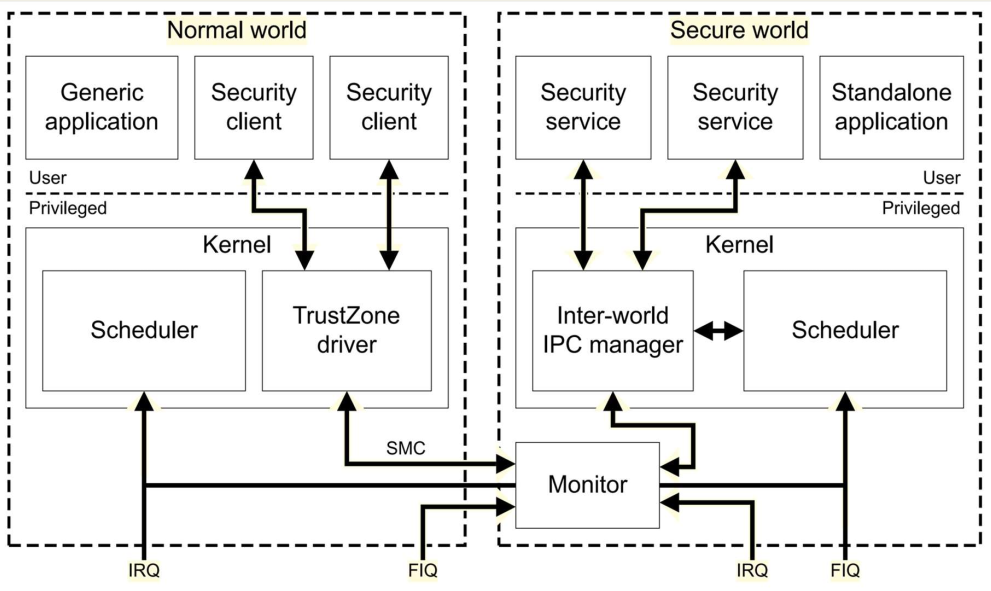
\includegraphics{images/TrustZone_secureOS.png}
   \caption{\textit{TrustZone} - Secure OS}
   \label{fig:trustzone_secureOS}
\end{figure}

\newpage
\section{Rogue Firmware}
An erroneous update or because of a malicious software developer, a device can store some malicious software that attacks the
system or offers an hidden backdoor.

Some run time attacks can be discovered by memory introspection or
attestation, other ones can be discovered by an \textit{host-based} Intrusion Detection System called \textbf{Doppelganger}.

A Doppelganger first analyzes the firmware of the \textit{embedded device} to detect
live code regions\footnote{executable parts of the firmware} therein, where it randomly
inserts its \textbf{symbiotes} (\textit{watchpoints}), and computes a CRC32 checksum of such randomly selected regions.

During the firmware execution, every time the \textit{symbiote manager}\footnote{Software that the Doppelganger adds \textit{before} the firmware} detects
a symbiote in memory,
\begin{enumerate}
   \item it stops the execution process (symbiote=breakpoint),
   \item compares the current memory area checksum of the symbiote one,
   \item Dopplganger considers a mismatch an evidence of a modification
   attack and it prevents the processor from running the code.
\end{enumerate}

\note{
   Doppelganger does not defend against attacks that load code in the dynamic memory
}

\section{Secure Management of a Device}
The manifacturer must flash bootstrap credentials onto the device,
which allow it to reach its "home" bootstrap sever.
Then it can ask such bootstrap server for a DM server address and the respective credentials,
to allow the DM server to manage the device.

\section{Encryption in IoT}
\textbf{Simon} and \textbf{Speck} are two families of block ciphers proposed by NSA,
with \texttt{SIMON} being tuned for optimal hardware performance, while \texttt{SPECK} for software.

Depending on the security level requested, they have different implementations varying block sizes:
e.g. \texttt{SIMON 64/128} refers to a \texttt{SIMON} variant of the cipher with a block size of \texttt{64 bits} and a key size of \texttt{128 bits}.

Their aim are \textit{generality} and \textit{simplicity},
to hopefully provide high performance even on future constrained platforms, whatever they may be.
Currently they can exploit also the capabilities of specific-purpose ASIC/FPGA boards;
furthermore, they provide low latency, ease of protection against side-channel attacks, and are efficient from a power consumption point-of-view,
making them a perfect fit for the IoT device industry.

Sadly, since NSA isn't completely trusted by many countries, \texttt{SIMON} and \texttt{SPECK} have not yet become an industry standard,
even if they have been tested by both NSA and academical researchers since 2014.